\documentclass[11pt]{exam}
\usepackage[empty]{fullpage}
\usepackage{amsmath}
\usepackage{tikz}
\usepackage{pgfplots}
\usepackage{soul}

\newcommand{\ds}{\displaystyle}
\newcommand{\on}{\operatorname}
\newcommand{\Var}{\operatorname{Var}}

\begin{document}
\subsection*{Midterm 2 Review \hfill Math 222}

\textit{These are problems similar to the ones that might be on midterm 2. Be sure to also review class workshops and problems from the textbook.}

\begin{questions}


\question A news article reports that ``Americans have differing views
on two potentially inconvenient and invasive practices that airports could implement to uncover
potential terrorist attacks." This news piece was based on a survey conducted among a random
sample of 1{,}137 adults nationwide, interviewed by telephone November 7-10, 2010, where one of
the questions on the survey was ``Some airports are now using `full-body' digital x-ray machines to
electronically screen passengers in airport security lines. Do you think these new x-ray machines
should or should not be used at airports?" Below is a summary of responses based on party
affiliation.

\begin{center}
\begin{tabular}{l|ccc|c} 
~ & Republican & Democrat & Independent & Total \\ \hline
Should & 264 & 299 & 351 & 914 \\ 
Should not & 38 & 55 & 77 & 170 \\ 
Don't know/No answer & 16 & 15 & 22 & 53 \\  \hline
Total & 318 & 369 & 450 & 1137
\end{tabular}
\end{center}



\begin{parts}
\part Identify the variables in this study. 
\begin{solution}
(i) party affiliation and (ii) opinions about full body scanners at airports.
\end{solution}
\vfill


\part If there was no association between the variables in the study, then what would the expected count be for the number of Republican voters who would say that the new x-ray machines ``should not be used"?
\begin{solution}
The expected count in any cell of a two way table is the row total times the column total divided by the table total.  In this case it is:
$$\frac{170 \cdot 318}{1137} = 47.5.$$
\end{solution}
\vfill

\part A chi-squared test for association with the data above has $\chi^2 = 4.3576$, df $= 4$, p-value $= 0.3598$.  Explain what that means about the association between the variables.  
\begin{solution}
The association between party affiliation and opinions on full-body scanners is not statistically significant.  There might not be an association in the population. 
\end{solution}
\vfill


\part The conclusion of the chi-squared test might be incorrect. If an error was made, was it a Type 1 or a Type 2 Error? Explain.
\begin{solution}
We might be making a Type 2 error (false negative).  
\end{solution}
\vfill
\end{parts}


\question Which option best describes the distribution shown in the normal quantile-quantile plot below?

\noindent
\begin{minipage}{0.48\textwidth}
\begin{choices}
\choice The distribution is roughly normal.
\choice The distribution is not normal, it is skewed right.
\choice The distribution is not normal, but it is roughly symmetric.
\CorrectChoice The distribution is not normal, it is skewed left.
\end{choices}
\end{minipage}
\hfill
%second column (no space between first and second column!)
\begin{minipage}{0.5\textwidth}
\includegraphics[scale=0.4]{../../../Semesters12-19/Spring18/Math222/qqplot1.png}
\end{minipage}
\newpage

\question Researchers studying the link between prenatal vitamin
use and autism surveyed the mothers of a random sample of children aged 24 - 60 months with
autism and conducted another separate random sample for children with typical development. The
table below shows the number of mothers in each group who did and did not use prenatal vitamins
during the three months before pregnancy (periconceptional period).

\begin{center}
\begin{tabular}{l|cc|c} 
~ & Autism & Typical development & Total \\ \hline
No vitamin & 111 & 70 & 181 \\ 
Vitamin & 143 & 159 & 302 \\ \hline
Total & 254 & 229 & 483
\end{tabular}
\end{center}

\begin{parts}
\part Draw a segmented bar graph that shows the row proportions for the two-way table above (it should have two bars, one for the vitamin group and one for the no vitamin group). 
\begin{solution}
\begin{center}
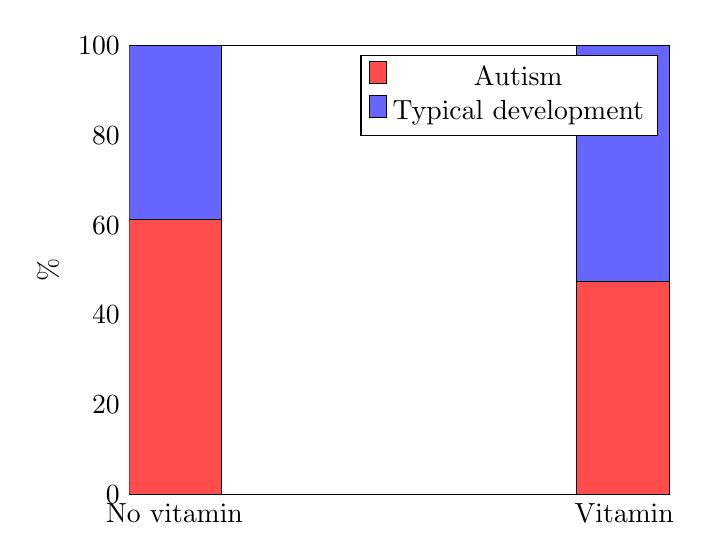
\begin{tikzpicture}
  \begin{axis}[
    ybar stacked,
    bar width=1.2cm,
    ymin=0, ymax=100,
    xtick=data,
    symbolic x coords={No vitamin, Vitamin},
    ylabel={\%},
    %legend style={at={(1.05,1)}, anchor=north west},
  ]

    % Red segments
    \addplot[fill=red!70] coordinates {
      (No vitamin, 61.3)
      (Vitamin, 47.4)
    };
    \addlegendentry{Autism}

    % Blue segments (remainder to reach 100)
    \addplot[fill=blue!60] coordinates {
      (No vitamin, 38.7)
      (Vitamin, 52.6)
    };
    \addlegendentry{Typical development}

  \end{axis}
\end{tikzpicture}
\end{center}
\end{solution}
\vfill

\part What are the correct null and alternative hypotheses if we want to see if there is a statistically significant difference between the proportions of kids with autism in the two groups?  Use symbols to write the hypotheses. 
\begin{solution}
\begin{itemize}
\item $H_0: p_\text{vitamin} = p_\text{none}$
\item $H_A: p_\text{vitamin} \ne p_\text{none}$
\end{itemize}
\end{solution}
\vfill
\part The R output of a 2-sample test for proportions with the data above is shown below.  As you can see, it includes a 95\% confidence interval.  Clearly explain what that confidence interval means in this situation.  
\begin{verbatim}
##  2-sample test for equality of proportions with continuity correction
## 
## data:  Autism 
## X-squared = 8.3131, df = 1, p-value = 0.003936
## alternative hypothesis: two.sided
## 95 percent confidence interval:
##  0.04475176 0.23474771
## sample estimates:
##    prop 1    prop 2 
## 0.6132597 0.4735099
\end{verbatim}
\begin{solution}
We can be 95\% sure that the autism rate is between 4.5\% and 23.5\% higher for children of mothers who did not take prenatal vitamins than for those who did.  
\end{solution}
\vfill
\part New York Times article reporting on this study was titled ``Prenatal Vitamins May Ward
Off Autism". Do you find the title of this article to be appropriate? Explain your answer.
Additionally, propose an alternative title.
\begin{solution}
The title suggests a causal relationship between prenatal vitamins and autism.  But that is not appropriate for an observational study.  Instead a better title would be ``Prenatal Vitamins are Associated with Fewer Autism Cases". 
\end{solution}
\vfill
\end{parts}



\newpage
\question Researchers interested in lead exposure due to car
exhaust sampled the blood of 52 police officers subjected to constant inhalation of automobile
exhaust fumes while working traffic enforcement in a primarily urban environment. The blood
samples of these officers had an average lead concentration of 124.32 $\mu$g/l and a SD of 37.74 $\mu$g/l;
a previous study of individuals from a nearby suburb, with no history of exposure, found an average
blood level concentration of 35 $\mu$g/l.
\begin{parts}
\part Write down the hypotheses that would be appropriate for testing if the police officers appear
to have been exposed to a higher concentration of lead.
\begin{solution}
\begin{itemize}
\item $H_0$: $\mu_\text{police} = 35$
\item $H_A$: $\mu_\text{police} \ne 35$
\end{itemize}
\end{solution}
\vfill
\part Explicitly state and check all conditions necessary for inference on these data.
\begin{solution}
The sample size is 52 which is large enough that we might be okay not worrying about normality, although we don't have any information about the shape of the distribution.  It doesn't say how the sample was collected, so there might be bias and issues with independence. 
\end{solution}
\vfill
\part Calculate the one-sample t-value needed to test the hypothesis that the downtown police officers have a higher lead exposure than the group in the previous study. 
\begin{solution}
$$t = \frac{124.32 - 35}{37.74 / \sqrt{52}} = 17.1.$$
\end{solution}
\vfill
\part Based on your preceding result, without performing a calculation, would a 95\% confidence
interval for the average blood concentration level of police officers contain 35 $\mu$g/l?
\begin{solution}
No, our results are 17.1 standard deviations above 35 $\mu$g/l.  A 95\% confidence interval would only extend about 2 standard deviations away from the sample mean $124.32$ $\mu$g/l.  So it definitely won't reach that far.  
\end{solution}
\vfill

\end{parts}

\question The National Center of Education Statistics conducted a survey of
high school seniors, collecting test data on reading, writing, and several other subjects. Here we examine a
simple random sample of 200 students from this survey. Side-by-side box plots of reading and writing scores
as well as a histogram of the differences in scores are shown below.
\begin{center}
\includegraphics[scale=0.28]{ex7-20.png}
\end{center}

\begin{parts}
\part Create hypotheses appropriate for the following research question: is there an evident difference in the
average scores of students in the reading and writing exam?
\begin{solution}
\begin{itemize}
\item $H_0: \mu_\text{reading} = \mu_\text{writing}$ or equivalently $\mu_\text{reading--writing} = 0$. 
\item $H_A: \mu_\text{reading} \ne \mu_\text{writing}$
\end{itemize}
\end{solution}
\vfill
\part Check the conditions required to complete this test.
\begin{solution}
The distribution of differences looks normal and the sample size is large, so we don't need to worry about the normality assumption. It says that the survey was a simple random sample so we can assume that sample bias won't be an issue.  Finally, the population of high school seniors is much larger than the sample, so our observations will be independent of each other.  
\end{solution}
\vfill
\newpage
\part The average observed difference in scores is $\bar{x}_\text{read--write} = -0.545$, and the standard deviation of the
differences is $8.887$ points.  What is the corresponding $t$-value, and how would you use the \verb|pt(t, df)| function in R to compute the corresponding p-value?  
\begin{solution}
The $t$-value is 
$$t = \frac{-0.545}{{8.887} / {\sqrt{200}}} = -0.867.$$
The corresponding p-value would be \verb|2 * pt(-0.876, df = 199)|. You need to multiply by 2 since we are testing a 2-sided alternative hypothesis.
\end{solution}
\vfill
\part Using the formula $\ds \bar{x} \pm t^* \sqrt{ s^2 + \frac{s^2}{n}}$ to make a 95\% prediction interval with this data, we get a range from $-18.1$ to $17.0$.  What are we 95\% sure will be between these two numbers?  
\begin{solution}
The prediction interval is 95\% likely to contain the differences in scores (reading minus writing) for any one random student in the population. Another way to say the same thing is that the differences in scores for 95\% of all students would fall in that range. 
\end{solution}
\vfill
\end{parts}

\question[6] In each of the following scenarios, determine whether it would be better to treat the data as matched pairs or as two separate samples.   
\begin{parts}
\part We would like to know if Intel's stock and Southwest Airlines' stock have similar rates of
return. To find out, we take a random sample of 50 days, and record Intel's and Southwest's share price on those same days. 
\begin{solution}
Matched pairs because the share prices are compared on the same days.
\end{solution}
\vfill
\part We randomly sample 50 items from Target stores and note the price for each. Then we visit
Walmart and collect the price for each of those same 50 items.
\begin{solution}
Matched pairs because the items are the same.
\end{solution}
\vfill
\part A school board would like to determine whether there is a difference in average SAT scores
for students at one high school versus another high school in the district. To check, they take
a simple random sample of 100 students from each high school. 
\begin{solution}
Two samples.  There two groups of students are independent random samples. 
\end{solution}
\vfill
\end{parts}

\newpage
\question A medical research group is recruiting people to complete short surveys
about their medical history. For example, one survey asks for information on a person's family history in
regards to cancer. Another survey asks about what topics were discussed during the person's last visit to a
hospital. So far, as people sign up, they complete an average of just 4 surveys, and the standard deviation
of the number of surveys is about 2.2. The research group wants to try a new interface that they think will
encourage new enrollees to complete more surveys, where they will randomize each enrollee to either get the
new interface or the current interface. The researchers are hoping that the new interface will increase the average number of completed surveys from 4 to 4.5.  
\begin{parts}
\part If the researchers enroll $n$ people to get the new interface and another $n$ people to get the old interface, then what R command would give the threshold for the two sample $z$-value 
$$z = \dfrac{\bar{x}_1 - \bar{x}_2}{\sqrt{\frac{\sigma_1^2}{n_1} + \frac{\sigma_2^2}{n_2}}}$$
to be statistically significant at the 5\% level? 
\begin{solution}
\verb|qnorm(0.95, mean = 0, sd = sqrt(9.68 / n))| since $\frac{2.2^2}{n} + \frac{2.2^2}{n} = \frac{9.68}{n}$. 
\end{solution}
\vfill
\part If the answer to the last part is stored in a variable called \verb|threshold|, then what R command can we use to find the power of the statistical test above (assuming a 1-sided alternative hypothesis, and an effect size of 0.5 extra surveys completed on average with the new interface)? 
\begin{solution}
\verb|1 - pnorm(threshold, mean = 0.5, sd = sqrt(9.8 / n))|
\end{solution}
\vfill
\end{parts}




\question A study of Canadian hockey players found that professional hockey players were far more likely to have birth months early in the year than later in the year.  Here is the data from players in the Western Hockey League in 1987.  
\begin{center}
\begin{tabular}{l|cccc|c}
\hline
Birth Month & Jan to Mar & Apr to Jun & Jul to Sep & Oct to Dec & Total \\ 
Count & 84 & 77 & 35 & 34 & 230\\ \hline
\end{tabular}
\end{center}
\begin{parts}
\part What statistical test would you do to see if there is a statistically significant difference in the birth months of hockey players than random chance alone would predict? 
\begin{solution}
Chi-squared test for goodness of fit.
\end{solution}
\vfill

\part What are the correct null and alternative hypotheses for this test? 
\begin{solution}
\begin{itemize}
\item $H_0:$ The proportion of hockey players in the population in each category are all the same. 
\item $H_0:$ The proportion of hockey players in the population in each category are not all the same. 
\end{itemize}
\end{solution}
\vfill

\part How many of the 230 players would you have expected to be born in each of the four categories if birthdates of hockey players were evenly distributed on the calendar?  
\begin{solution}
You would expect about 1/4 of the 230 players to be in each category, so 57.5 in each.
\end{solution}
\vfill
\end{parts}

\end{questions}


\end{document}
